\section{Machine Learning -- Theory}

\paragraph{}
	Machine learning, a branch of artificial intelligence, concerns the construction and study of systems that can learn from data \cite{wiki:machineLearning}. The supervised classification problem in machine learning concerns finding the unknown target function that classifies certain input data into classes based on some set of training examples containing labelled input data.
	
\paragraph{}
	In our case, given a sampled sound signal of a sleeper, we want to identify apnoea periods. In particular, we represent our input (sampled sound signal) as $\left\{s_1, s_2, \dotsc, s_T \right\} \equiv \left\{ s_i \right\}_{i = 1}^{T}$, and we want to output the classifiers for every $K$ samples, $\left\{ y_i \right\}_{i = 1}^{T/K}$, where the classifier $y_i \in \left\{0, 1\right\}$ corresponds to samples $\left\{ s_j \right\}_{j = \left(i - 1\right)K + 1}^{iK}$ of the signal. We assume that $T$ is divisible by $K$, however if this is not the case, we discard an appropriate number of signal samples to make it so.
	
\paragraph{}
	We have researched three models for our problem which we will discuss in this section. Firstly, we will discuss Support Vector Machines which are one of the most widely used algorithms in Machine Learning today, then we will discuss the State-Space and Hidden Markov Models, which turn out to be more well-suited to our problem due to their temporal nature. Moreover, we discuss techniques to condition our data before using them as input data for our learning models.
	
\subsubsection{Support Vector Machines}
\subsubsection*{State-Space Models}

\paragraph{}
	Here, we present the State-Space Models (SSMs) (also known as Linear Dynamical Systems) based on Kevin Murphy's book \cite[Chapter 18]{mlBook}. SSMs allow us to model systems that are dynamic. Unlike the SVMs, SSMs will model dependencies of the current state on the previous ones.
\subsection{Hidden Markov Models}

\paragraph{}
	Here, we present the Hidden Markov Models (HMMs), one of the most popular statistical models in machine learning with applications in many fields including but not limited to Cryptanalysis, Speech recognition and Bioinformatics \cite{wiki:HMM}. The material presented here is based on \cite{rabiner1989tutorial}, \cite{ramage07} and \cite{mlBook}. We will first present HMMs with discrete observations, then we extend this to include models with continuous observations.
	
\subsubsection{Discrete observations}
\paragraph{}
	Similarly to SSMs, we have two sets of random variables. Observed variables $\vec Y = \{ y_t \}_{t = 1}^T$ which are drawn from the observation alphabet $V = \{v_1, \dotsc, v_M\}$, and hidden states $\vec X = \{ x_t \}_{t = 1}^T$ which are drawn from the hidden state alphabet $S = \{ s_1, \dotsc, s_N \}$. The probabilistic graphical model of the HMM is identical to the one in Figure \ref{fig:pgm}. The hidden states obey Markov assumptions, i.e. $P( x_t | x_{t - 1}, \dotsc, x_1) = P(x_t | x_{t - 1}) = \text{const.}, t = 2, \dotsc, T$. Moreover, the observed variables are only dependent on the corresponding hidden state, i.e. $P( y_t | x_t, \dotsc, x_1, y_{t - 1}, \dotsc, y_1) = P(y_t | x_t), t = 1, \dotsc, T$.
	
\paragraph{}
	We parameterise a HMM using the transition matrix $\vec A$, emission matrix $\vec B$, and the initial state distribution $\vec \pi$. The transition matrix $\vec A \in \mathbb{R}^{N \times N}$ describes the transitions between hidden states, $A_{ij} = P(x_{t + 1} = s_j | x_t = s_i)$. The emission matrix $\vec B \in \mathbb{R}^{N \times M}$ describes the probability of an observation conditioned on a hidden state, $B_{jk} = B_{j}(v_k) = P(y_t = v_k | x_t = s_j)$. The initial state distribution $\vec \pi \in [0, 1]^N$ simply describes the initial probabilities of the hidden state, $\pi_i = P(x_1 = s_i)$. The model is fully described if we know these parameters, which we group into what is called a parameter set of the model, $\lambda = (\vec A, \vec B, \vec \pi)$.
	
\paragraph{}
	The three main questions of a HMM are
	\begin{enumerate}
		\item Find the probability of observations given the model, $P\left(\vec Y; \lambda\right)$.
		\item Find the most likely series of hidden states $\vec X$ to have generated the observations $\vec Y$, $\vec X^\ast = \argmax_{\vec X} P\left(\vec Y | \vec X; \lambda\right)$.
		\item Find the parameters $\lambda$ to maximise $P\left(\vec Y; \lambda\right)$.
	\end{enumerate}
We will discuss algorithmic solution to these three problems in turn.

\paragraph{Solution to the first problem.} To find the probability of an observed sequence, we use the dynamic programming algorithm, called the \textsc{Forward procedure} (outlined in Algorithm \ref{alg:forward}) which calculates the forward variable $\alpha_t (i) = P(\vec Y, x_t = s_i; \lambda)$.
\begin{algorithm}
	\caption{\textsc{Forward Procedure} for computing $\alpha_t(i)$.}
	\label{alg:forward}
	\begin{enumerate}
		\item
			\textbf{Initialisation.}
			$$\alpha_1(i) = \pi_i B_i(y_1), 1 \leq i \leq N$$
		\item
			\textbf{Induction.}
			\begin{equation*}
				\alpha_{t + 1}(j) = \left[ \sum_{i = 1}^N \alpha_t(i) A_{ij} \right] B_j (y_{t + 1}), 
				\begin{array}{lr}
					1 \leq t \leq T - 1\\
					1 \leq j \leq N
				\end{array}
			\end{equation*}
			
		\item
			\textbf{Termination.} (solution to the first problem)
			$$P\left(\vec Y; \lambda\right) = \sum_{i = 1}^N \alpha_T(i)$$
	\end{enumerate}
\end{algorithm}
As we can see, the algorithm has a time complexity of $O(TN)$.

\paragraph{Solution to the second problem.} 
	To solve the problem of finding the most likely sequence of hidden states, we use the \textsc{Viterbi Algorithm} proposed by Andrew Viterbi in 1967. The most likely sequence of hidden states is also called the Viterbi path. Firstly, we define the quantity $\delta_t(i)$, which stores the highest probability along a single path ending at the state $x_t = s_i$:
	\begin{equation}
		\delta_t(i) = \max_{x_1, \dotsc, x_{t - 1}} P\left( x_1, \dotsc, x_{t - 1}, x_t = s_i, y_1, \dotsc, y_t; \lambda \right)
	\end{equation}
By induction, we have
	\begin{equation}
		\delta_{t + 1}(j) = \left[ \max_i \delta_t(i) A_{ij} \right] B_j(y_{t + 1})
	\end{equation}
We also keep track of the index of the hidden state that maximises this quantity in
	\begin{equation}
		\psi_{t + 1}(j) = \argmax_i \delta_t(i) A_{ij}
	\end{equation}
Having defined these quantities, we present the \textsc{Viterbi Algorithm} in Algorithm \ref{alg:viterbi}.
\begin{algorithm}
	\caption{\textsc{Viterbi Algorithm} for computing the most likely sequence of hidden states.}
	\label{alg:viterbi}
	\begin{enumerate}
		\item
			\textbf{Initialisation.}
			\begin{align*}
				\delta_1(i) & = \pi_i B_i(y_1), & 1 \leq i \leq N \\
				\psi_1(i) & = 0, & 1 \leq i \leq N
			\end{align*}
		\item
			\textbf{Recursion.}
			\begin{align*}
				\delta_t(j) & = \max_{1 \leq i \leq N} \left[ \delta_{t - 1}(i) A_{ij} \right] B_j(y_t), &
				\begin{array}{lr}
					2 \leq t \leq T\\
					1 \leq j \leq N
				\end{array}\\
				\psi_t(j) & = \argmax_{1 \leq i \leq N} \left[ \delta_{t - 1}(i) A_{ij} \right], &
				\begin{array}{lr}
					2 \leq t \leq T\\
					1 \leq j \leq N
				\end{array}
			\end{align*}
		\item
			\textbf{Termination.}
			\begin{align*}
				P^\ast & = \max_{1 \leq i \leq N} \delta_T(i)\\
				x_T^\ast & = \argmax_{1 \leq i \leq N} \delta_T(i)
			\end{align*}
		\item
			\textbf{Path backtracking.}
			\begin{equation*}
				x_t^\ast = \psi_{t + 1}\left(x_{t + 1}^\ast \right),  T - 1 \geq t \geq 1
			\end{equation*}
		\item
			\textbf{Return $\left\{x_t^\ast \right\}_1^T$.}
	\end{enumerate}
\end{algorithm}
As we can see, the algorithm has a time complexity of $O(TN^2)$.

\paragraph{Solution to the third problem.}
	To learn the parameters of the model, $\lambda = \left( \vec A, \vec B, \vec \pi \right)$, we use the \textsc{Forward-Backward Algorithm} by Baum-Welch. We will need to introduce few quantities. Firstly, we introduce the backward variable $\beta_t(i) = P\left( y_{t + 1}, \dotsc, y_T | x_t = s_i; \lambda \right)$ which can be computed using a dynamic programming algorithm in Algorithm \ref{alg:backward}.
	\begin{algorithm}
		\caption{\textsc{Backward Algorithm} for computing $\beta_t(i)$.}
		\label{alg:backward}
		\begin{enumerate}
			\item
				\textbf{Initialisation.}
				$$\beta_T(i) = 1, 1 \leq i \leq N$$
			\item
				\textbf{Induction.}
				\begin{equation*}
					\beta_t(i) = \sum_{j = 1}^N A_{ij} B_j(y_{t + 1}) \beta_{t + 1}(j), 
					\begin{array}{lr}
						T - 1 \leq t \leq 1\\
						1 \leq j \leq N
					\end{array}
				\end{equation*}
		\end{enumerate}
	\end{algorithm}
We also define the variable $\gamma_t(i) = P\left( x_t = s_i | \vec Y; \lambda \right)$ which can be expressed as
	\begin{align}
		\gamma_t(i) 	& = P\left( x_t = s_i | \vec Y; \lambda \right) \nonumber\\
				& = \frac{ P\left( x_t = s_i, \{ y_\tau \}_1^t; \lambda \right)  P\left( \{ y_\tau \}_{t + 1}^T | x_t = s_i; \lambda \right)}{ P\left( \vec Y; \lambda \right)} \nonumber\\
				& = \frac{\alpha_t(i) \beta_t(i)}{\sum_{i = 1}^N \alpha_t(i) \beta_t(i)} \label{eqn:hmmGamma}
	\end{align}
We also define the quantity $\xi_t(i, j)$ as
	\begin{align}
		\xi_t(i, j) 	& = P\left(x_t = s_i, x_{t + 1} = s_j | \vec Y; \lambda \right) \nonumber\\
				& = \frac{\alpha_t(i) A_{ij} B_j(y_{t + 1}) \beta_{t + 1}(j)}{\sum_{i, j = 1}^N \alpha_t(i) A_{ij} B_j(y_{t + 1}) \beta_{t + 1}(j)}
	\end{align}
Now, we are in a position to present the \textsc{Forward-Backward Algorithm} by Baum-Welch in Algorithm \ref{alg:baumwelch}. The algorithm belongs to a family of Expectation-maximisation (EM) algorithms for finding maximum likelihood (ML) or maximum a posteriori (MAP) estimates of parameters in statistical models \cite{wiki:EM}.
\begin{algorithm}
	\caption{\textsc{Forward-Backward Algorithm (Baum-Welch)} for estimating HMM parameters $\lambda$.}
	\label{alg:baumwelch}
	\begin{enumerate}
		\item
			\textbf{Initialisation.}
			Set $\vec A$, $\vec B$, $\vec \pi$ to be random valid probability matrices/vectors.
		\item
			\textbf{Repeat until convergence:}
			\begin{itemize}
				\item \textbf{E-step.} Run \textsc{Forward} and \textsc{Backward Procedures} to get $\alpha_t(i)$ and $\beta_t(i)$. Evaluate $\gamma_t(i)$ using \eqref{eqn:hmmGamma}.
				\item \textbf{M-step.} Re-estimate parameters using
				\begin{align*}
					\pi_i & = \gamma_1(i) \\
					A_{ij} & = \frac{\sum_{t = 1}^{T - 1} \xi_t(i, j)}{\sum_{t = 1}^T \gamma_t(i)} \\
					B_j(v_k) & = \frac{\sum_{t = 1, \text{s.t.} y_t = v_k}^T \gamma_t(j)}{\sum_{t = 1}^T \gamma_t(j)}
				\end{align*}
			\end{itemize}
	\end{enumerate}
\end{algorithm}

\paragraph{Parameters estimation with known hidden states.} In case the hidden states $\vec X$ are given to us, in addition to the observed variables $\vec Y$, the problem of parameters estimation simply reduces to counting transitions, i.e.
	\begin{align}
		A_{ij} & = \frac{\sum_{t = 1}^{T - 1} 1\{x_t = s_i \land x_{t + 1} = s_j\}}{\sum_{t = 1}^{T} 1\{x_t = s_i\}} \\
		B_j(k) & = \frac{\sum_{t = 1}^T 1\{x_t = s_j \land y_t = v_k\}}{\sum_{t = 1}^{T} 1\{x_t = s_j\}}
	\end{align}
where $1(\cdot)$ is an indicator function ($1$ if the boolean argument is true, $0$ otherwise).

\subsubsection{Continuous observations}

\paragraph{}
	We now discuss the case in which the observations $\vec Y = \{y_t\}_1^T$ are not drawn from a finite set $V$, but are real-valued vectors $\{\vec y_t\}_1^T$, drawn from $\mathbb{R}^d$, i.e. $\vec y_t \in \mathbb{R}^d, 1 \leq t \leq T$ (Note: hidden states $\vec X = \{x_t\}_1^T$ are still drawn from a finite set $S$). In this case, we cannot describe the observations using an emission matrix anymore. Since the observation random variables are now continuous, they must be drawn from some probability distribution function (pdf). This function can be any arbitrary pdf, however in order to learn anything useful, we parameterise it. We assume a simple case and let it be a Gaussian, parameterised by its mean, and covariance. In particular, $B_j(\cdot)$ becomes a probability distribution function:
	\begin{align}
		B_j(\vec y_t) 	& = P\left( \vec y_t | x_t = s_j\right) \nonumber\\
					& = \mathcal{N}(\vec y_t; \vec\mu_j, \vec U_j), \label{eqn:gaussian}&
		\begin{array}{lr}
			1 \leq t \leq T\\
			1 \leq j \leq N
		\end{array}
	\end{align}
This means that instead of the original emission matrix $\vec B$, we are now parameterising the emissions using the means $\vec\mu = \{\vec\mu_j \in \mathbb{R}^d\}_1^N$ and the covariances $\vec U = \{\vec U_j \in \mathbb{R}^{d\times d}\}_1^N$. Thus, our parameters set becomes $\lambda = \left\{ \vec A, \vec \mu, \vec U, \vec \pi\right\}$.

\paragraph{Changes to the algorithms.}
	While the three main questions for the HMM remain the same, we must change the algorithms used in the discrete observations case. It turns out that in the \textsc{Forward Procedure} (Algorithm \ref{alg:forward}), \textsc{Backward Procedure} (Algorithm \ref{alg:backward}), and the \textsc{Viterbi Algorithm} (Algorithm \ref{alg:viterbi}), we don't need to change anything except the interpretation of $B_j(\cdot)$. Whereas before, we had a single value for this quantity, now we must evaluate it using the parameters of the pdf (in this case mean and covariance) in \eqref{eqn:gaussian}. The problem of estimating parameters, given the observations becomes slightly different and will be left untouched in our report. However, we discuss parameters estimation, given both the observations and the hidden states, which simply becomes fitting a Gaussian, i.e.
	\begin{align}
		\vec\mu_j & = \frac{\sum_{t = 1}^T 1\{x_t = s_j\} \vec y_t}{\sum_{t = 1}^T 1\{x_t = s_j\}} \\
		\vec U_j & = \frac{\sum_{t = 1}^T 1\{x_t = s_j\} (\vec y_t - \vec\mu_j)(\vec y_t - \vec\mu_j)^T}{\sum_{t = 1}^T 1\{x_t = s_j\}}
	\end{align}

\paragraph{Different probability density functions.}
	We have assumed that the conditional distribution of the observations is Gaussian. One disadvantage of this method is that it may be too simple to capture the real pdf the observations are drawn from. One of the alternatives is the Gaussian Mixture Model (GMM), however fine-tuning the number of modes can be difficult. It turns out that finding the optimal MLE for a GMM is intractable \cite{mlBook}.
	
\subsubsection{Our problem}
\paragraph{}
	In our problem, we model the apnoeatic states as the hidden states $\{x_t\}_1^T$ drawn from a binary set $\{0, 1\}$. Although the observed signal is a sampled one-dimensional signal, since we only have annotations every $K$ samples, we stack all $K$ samples to a vector and treat it as a $K$-dimensional, real-valued observed variable $\vec y_t \in \mathbb{R}^d$, ($d = K$). Since we assume that we have the annotated signal, we can do the training offline. Thus we are interested in the third problem (with known hidden states), for which the solution is just fitting the parameters; and the second problem, finding the most likely sequence of the apnoeatic diagnoses, given the model and the observations, using the \textsc{Viterbi Algorithm}. We will train the model using the annotated data and once trained, we will use the trained model to diagnose sleep apnoea from new data. Implementations of the algorithms for our applications are available for \verb!MATLAB!\textsuperscript{\textregistered} in the packages \verb!pmtk3! (\url{https://github.com/probml/pmtk3}) and \verb!HMM Toolbox! (\url{http://www.cs.ubc.ca/~murphyk/Software/HMM/hmm.html}) from Kevin Murphy.
\subsection{Conditioning input data}
	Working in the time domain, the data is usually transformed to the frequency domain to analyse where the pattern is found more easily. Also, ergardless of the chosen model, we will work in high dimensions which means we need a lot of input data in order to find the pattern. In the case of SVMs, it will be high-dimensional training points $\{\vec x^{(i)}\}_1^m$; in the case of SSMs and HMMs, it will be the high-dimensional observed variables $\{\vec y_t\}_1^T$. We will present two ways to condition the input data, before analysing it using the learning algorithms above, namely frequenc-domain analysis and Principal Components Analysis.
	
	\subsubsection{Frequency-domain analysis}
		\paragraph{Discrete Fourier Transform.}
			Discrete Fourier Transform (DFT) is used to transform a finite list of equally spaced samples of a function into the list of coefficients of a finite combination of complex sinusoids \cite{wiki:DFT}. It can be said to convert the sampled function from its original domain to the frequency domain \cite{wiki:DFT}. The DFT, $\mathcal{F}$, can be defined to transform $\vec x = \{x_1, x_2, \dotsc, x_{N}\}$ to $\vec X = \{X_1, X_2, \dotsc, X_{N}\}$ as
			\begin{equation}
				X_k = \sum_{n = 1}^{N} x_n \exp{(-i2\pi k n / N)}, 1 \leq k \leq N
			\end{equation}
			and can be performed using the Fast Fourier Transform (FFT) algorithm.

		\paragraph{Power Spectral Density.}
			It is common to take the Power Spectral Density (PSD) instead of the DFT in order to remove the imaginary components in the frequency domain. The PSD of a continuous signal $x(t)$ can be defined as
			\begin{equation}
				S_{xx}(f) = \lim_{T \to \infty} \frac{1}{T} \left| X(f) \right|^2
			\end{equation}
			where $X(f)$ is the Fourier transform ($\mathcal{FT}$) of $x(t)$ in the interval $-T / 2 < t < T / 2$ \cite{hlt}. It can be shown that in the discrete case where $\vec x = \{x_1, x_2, \dotsc, x_{N}\}$, the PSD is obtained by
			\begin{align}
				S_{xx}(k) 	&= \lim_{T \to \infty} \frac{(\Delta t)^2}{T} |X_k|^2\\
							&\approx \frac{(\Delta t)^2}{T} |X_k|^2
			\end{align}
			where $T$ is the actual recording time, $N$ is number of samples and $1/\Delta t$ is the sampling frequency (note that $T = N(\Delta t)$) \cite{wiki:PSD}.

		\paragraph{Spectrograms.}
			To create a spectrogram of a signal $\vec x = \{x_1, x_2, \dotsc, x_N\} = \{x(\Delta t), x(2\Delta t), \dotsc, x(N\Delta t)\}$, we must choose a window size $T_\text{window}$ and an offset $T_\text{offset}$. Then, we keep shifting the window by $T_\text{offset}$ and each time, we transform and store the window's content (in time domain) to the frequency domain using the DFT. This way, we will have a frequency domain data of the size $T_\text{window}$ every $T_\text{offset}$, which we will call $\vec X_1, \vec X_2, \dotsc, \vec X_\tau$. We usually represent this frequency domain data using colour intensities and plot them as $\tau$ columns of colour intensities with time on the horizontal axis and frequency on the vertical axis. Figure \ref{fig:spec} illustrates the process of creating a spectrogram. However, it is common to find the PSDs instead of the DFTs of the sliding windows (the principle stays the same). Hence we will refer to the process of creating the spectrogram with PSDs (instead of DFTs) of the sliding windows as \emph{freqency analysis of the signal}.
			\begin{figure}[h!]
				\centering
					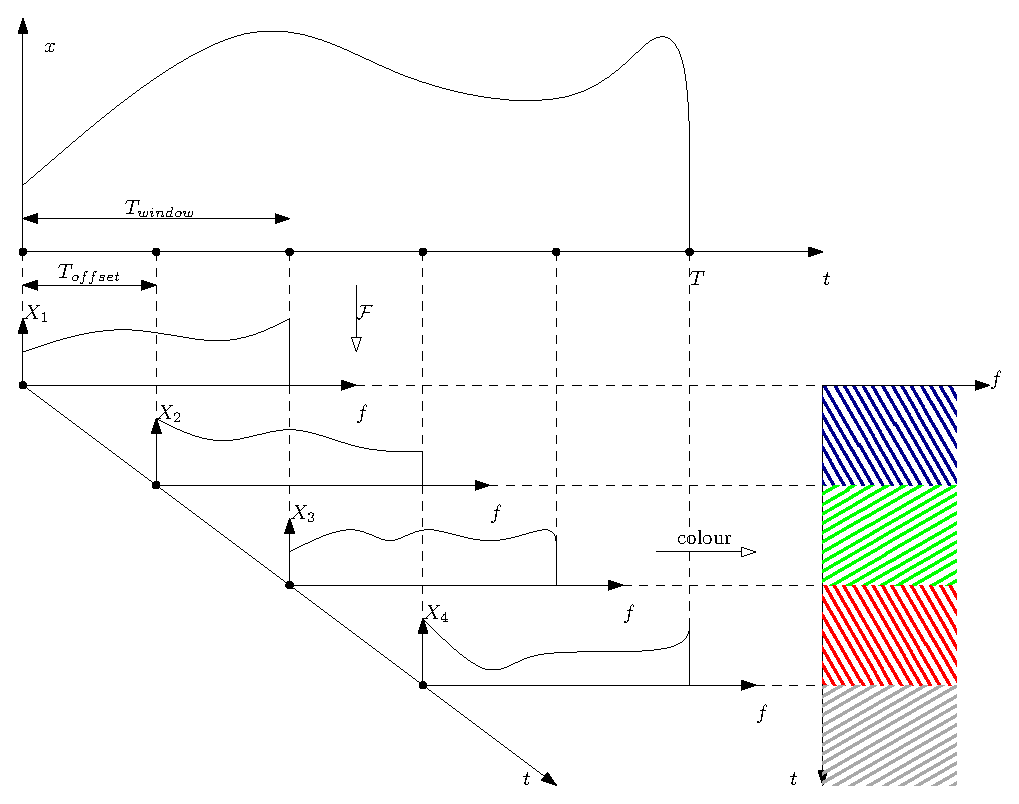
\includegraphics{drawings/spec.eps}
				\caption{The process of creating a spectrogram.}
				\label{fig:spec}
			\end{figure}

	\subsubsection{Principal Components Analysis}
		Here we present the theory for Principal Components Analysis (PCA) based on Andrew Ng's lecture notes \cite{ng13} and Kevin Murphy's book \cite{mlBook}. The objective is to take $m$ $n$-dimensional input data points $\{\vec x^{(i)} \in \mathbb{R}^n\}_1^m$ and transform them into $m$ $k$-dimensional data points ($k<n$) $\{\vec y^{(i)} \in \mathbb{R}^m\}_1^m$, where $\vec y^{(i)}$'s are projections of $\vec x^{(i)}$'s onto $k$ orthonormal basis vectors $\{\vec u_i\}_1^k$ while ``preserving the most variance''. We assume that over all $m$ points, their $\text{mean}\left[\{x^{(i)}_j\}_{i = 1}^m\right] = 0$ and their $\text{var}\left[\{x^{(i)}_j\}_{i = 1}^m\right] = 1$ for all features of the input points $1 \leq j \leq n$. We normalise the data first if this is not the case. For $n = 2$, $k = 1$, Figure \ref{fig:pca} shows the projections to the new axis.
		\begin{figure}[h!]
			\centering
				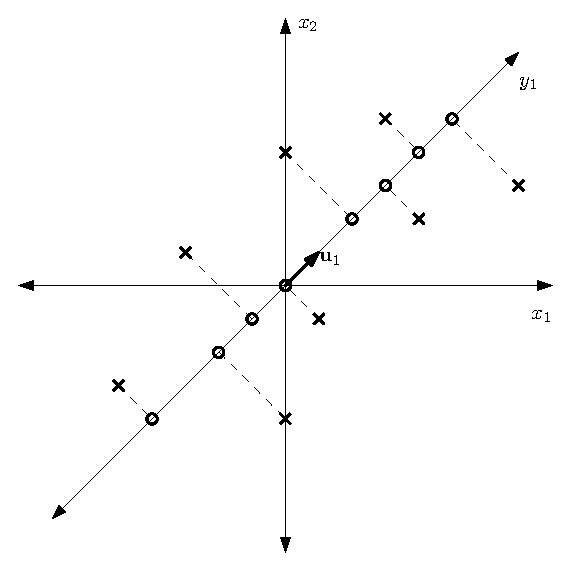
\includegraphics{drawings/pca.eps}
			\caption{Illustration of PCA.}
			\label{fig:pca}
		\end{figure}

		We can see that the transformed points can be expressed as
		\begin{equation}
		 	\vec y^{(i)} =
		 		\begin{bmatrix}
		 			\vec u_1^T \vec x^{(i)} \\
		 			\vec u_2^T \vec x^{(i)} \\
		 			\vdots \\
		 			\vec u_k^T \vec x^{(i)} \\
		 		\end{bmatrix}
		 		, 1 \leq i \leq m
			\label{eqn:pca}
		\end{equation}
		
		It can be shown that in order to maximise $\sum_{i = 1}^m \left\| \vec y^{(i)} \right\|^2$, conditioned on orthonormality of the bases, we must choose normalised eigenvectors corresponding to the $k$ largest eigenvalues of the variance matrix $\vec \Sigma = \frac{1}{m} \sum_{i = 1}^m \vec x^{(i)} {\vec x^{(i)}}^T$ as the bases. These bases are also called the \emph{principal components}. The eigenvalues are proportional to the actual variances of data in the new bases. Hence, we can compare the relative ``importance'' of the bases and use this fact to decide how many principal components to use.